\documentclass[journal]{IEEEtran}

\usepackage{cite}
\usepackage{amsmath}
\usepackage{graphicx}
\usepackage{booktabs}
\usepackage{hyperref}
\usepackage{url}
\usepackage{tabularx}
\usepackage{tfrupee}
\usepackage{tikz}
\usepackage{float}
\usepackage{subcaption}
\usetikzlibrary{shapes.geometric, arrows.meta, positioning, calc}

% === TikZ Workflow Styles (IEEE column-width safe) ===
\tikzset{
  wf node/.style={
    rectangle, rounded corners=2pt, draw=black, fill=gray!8,
    text width=1.3cm, minimum height=0.65cm,
    text centered, font=\sffamily\scriptsize,
    inner sep=2pt
  },
  wf trigger/.style={
    wf node, fill=gray!20, font=\sffamily\scriptsize\bfseries
  },
  wf decision/.style={
    diamond, draw=black, fill=gray!8,
    text width=0.7cm, minimum height=0.5cm,
    text centered, font=\sffamily\scriptsize,
    inner sep=1pt, aspect=2.2
  },
  wf arrow/.style={
    -Stealth, thick, draw=black!70
  },
  wf label/.style={
    font=\sffamily\tiny, fill=white, inner sep=1pt
  }
}

\hypersetup{
    colorlinks=false,
    pdfborder={0 0 0},
}

\begin{document}

\title{StockSense AI: An Intelligent Inventory Management and Supplier Decision Support System for Small Retail Stores}

\author{Vyshakh Vijayan%
\thanks{Vyshakh Vijayan is with the Department of Computer Science and Business Systems, VIT-AP University, Amaravati, Andhra Pradesh, India. Email: vijayan.22bcb7055@vitapstudent.ac.in}%
}

\markboth{StockSense AI Project Report}%
{Vyshakh Vijayan: StockSense AI: Intelligent Inventory Management for Small Retail Stores}

\maketitle

\begin{abstract}
India has over 12 million kirana stores, and most of them still track inventory by hand. Expensive enterprise software is out of reach for these shop owners, so they end up guessing when to reorder stock. StockSense AI addresses this gap. It is a web-based inventory intelligence system that runs on mostly free-tier cloud services and costs under Rs.~500 a month in production. The architecture has four layers: a React~19 frontend, Supabase PostgreSQL for storage, n8n for workflow automation, and Groq Llama~3.1~8B for generating reorder suggestions. Every morning at 8:00~AM IST, a master workflow runs eight sub-pipelines that calculate stockout dates, classify risk levels, score suppliers with a Weighted Sum Model, produce AI-driven reorder recommendations, and push a summary to the store owner's WhatsApp via Twilio. Testing with six products and three suppliers shows that the full pipeline finishes in roughly 13 seconds, alerts arrive within 5 seconds, and the health-score formula behaves as expected across extreme inventory states.
\end{abstract}

\begin{IEEEkeywords}
Inventory Management, Supply Chain Intelligence, Workflow Automation, n8n, Large Language Model, Supplier Scoring, Kirana Stores, SME Technology
\end{IEEEkeywords}

\section{Introduction}
\IEEEPARstart{W}{alk} into any kirana store in India and you will notice the same thing---the owner tracks stock in a notebook or, at best, a basic spreadsheet. With over 12 million such neighborhood shops in the country, this manual approach leads to two recurring problems. Either the shelves run empty and customers leave, or money sits locked in unsold inventory. Both outcomes eat into already thin margins.

Why does this persist? For one, enterprise software such as Zoho Inventory starts at Rs.~4,000 a month, which is impractical for a shop earning Rs.~15,000--20,000 in monthly profit. Simpler POS apps like Khatabook and Vyapar do exist, but they only record past sales---they cannot predict what will run out next week or suggest how much to reorder. On top of that, Indian supply chains are fragmented: a single store may deal with five to ten suppliers, each with different reliability and delivery speeds, making vendor selection a daily guessing game.

StockSense AI was built to fill this exact gap. It is an end-to-end inventory intelligence system for small Indian retailers, and it runs on mostly free-tier cloud services. The five goals driving the project are: (1)~track stock in real time and predict upcoming stockouts, (2)~generate reorder suggestions using a large language model, (3)~rank suppliers through a Weighted Sum Model, (4)~send WhatsApp alerts automatically, and (5)~keep the total cost under Rs.~500 per month.

What makes this work different from a typical inventory app is the automation layer. Every morning at 8:00~AM, a master orchestration workflow triggers eight sub-pipelines that update stockout dates, flag risky products, call the Groq Llama~3.1~8B model for reorder reasoning, score suppliers, and finally push a WhatsApp digest to the shop owner. The store owner does not need to open the dashboard at all---the system comes to them.

The rest of this paper is laid out as follows. Section~II reviews related work. Section~III explains the motivation and problem specification. Section~IV describes the architecture and mathematical models. Section~V covers implementation details. Section~VI discusses results, and Section~VII concludes with future scope.

\section{Related Work}

Several lines of research inform the design of StockSense~AI. This section groups them into four themes: smart inventory systems, demand forecasting, LLM-based decision support, and workflow automation.

On the inventory systems front, Wang et~al.~\cite{inventory2024} built an intelligent warehousing system for small enterprises and reported clear gains in stock accuracy. Their paper also noted, however, that adoption among micro-retailers stays low because even ``affordable'' solutions assume internet literacy and upfront hardware. This observation matches what we see in Indian kirana stores, where the owner is often the sole employee.

Forecasting is a well-studied area. Kheawpeam and Sinthupinyo~\cite{forecasting2023} showed that ML models beat traditional moving-average methods by 15--25\% for multi-channel retailers. Soni and Vaghela~\cite{retail2024} extended this by adding external signals like festivals and promotions. Both studies, though, target organized retail chains with historical POS data spanning months. A kirana shop that has never digitized its sales does not have that data, which is why StockSense currently relies on a simpler rule-based stockout formula rather than trained ML models.

Large language models are beginning to appear in business decision-making. Al~Khaldy and Gheraibia~\cite{llm2024} evaluated GPT-class models on procurement tasks and found them useful but prone to hallucination. Friedman et~al.~\cite{cognitive2025} took a different angle, showing that LLM suggestions can reduce cognitive biases in purchasing decisions. We draw on both findings: StockSense uses Groq Llama~3.1~8B for reorder reasoning, but wraps it with a rule-based fallback so that a malformed API response never breaks the pipeline.

Workflow automation has quietly become central to small-business IT. Amir and Atif~\cite{workflow2025} benchmarked n8n against manual processes and found it cut implementation time significantly. Venkiteela~\cite{n8n2025} positioned n8n as a viable alternative to Zapier for enterprise integration. Our choice of n8n over a custom backend is driven by these findings---it lets one developer wire together eight workflows without writing server-side code.

On the supplier-evaluation side, Weighted Sum Model (WSM) approaches are standard in operations research. StockSense applies WSM with three criteria---reliability, price competitiveness, and delivery speed---weights that were chosen after reviewing common small-retailer priorities.

Finally, hardware-centric approaches deserve mention. Manoharan et~al.~\cite{iot2024} combined IoT sensors with ML for automated stock counting, and Poongothai et~al.~\cite{smartretail2024} proposed smart-retail forecasting. Both require RFID readers or IoT gateways, which adds Rs.~10,000--50,000 in upfront cost. For a kirana store, that is a non-starter. Shenoy and Mal~\cite{msme2019} specifically studied Indian MSME inventory needs and called for ``simple yet effective'' tools---an ethos StockSense tries to follow by keeping the entire stack software-only.

\section{Motivation and Problem Specification}

There is a wide gulf between what the research community proposes and what a kirana store owner can actually use. Most published inventory models assume clean historical data, stable internet, and a dedicated IT person---none of which exist in a typical neighborhood shop.

\subsection{Socio-Economic Motivation}
Kirana stores account for roughly 80\% of India's grocery retail, yet almost none of them use any digital tool beyond a UPI payment app. A single stockout---say, running out of Aashirvaad Atta during a festival week---can send a loyal customer to the competitor across the street. On the flip side, over-ordering perishable goods like bread or milk leads to waste. Both mistakes directly hit the owner's pocket. StockSense AI was motivated by this everyday pain point: can we give a small shopkeeper the kind of stock intelligence that a Reliance Fresh or DMart gets from its ERP, but without the cost?

\subsection{Gap Analysis and Technical Advantage}
Two specific gaps stood out during our literature review and field observations:
\begin{enumerate}
    \item \textbf{Financial Barrier}: ``Smart'' inventory systems typically need RFID hardware or carry SaaS subscriptions costing Rs.~500--5,000 per month. StockSense keeps costs under Rs.~500/month by stitching together free-tier services---Supabase for the database, Groq for LLM inference, and a locally hosted n8n instance for automation. Enterprise tools like Zoho Inventory cost Rs.~4,000+ for comparable features.
    \item \textbf{Intelligence Gap}: Apps like Vyapar and Khatabook are popular but reactive---they tell the owner what \textit{was} sold, not what \textit{will} run out. By plugging in an 8B-parameter language model, StockSense brings reasoning-based reorder logic to a segment that has never had it.
\end{enumerate}

\subsection{Problem Statement}
The goal is straightforward: build a pipeline that takes raw inventory numbers, figures out which products are at risk, decides how much to reorder and from which supplier, and delivers the recommendation to the owner's WhatsApp---all without the owner lifting a finger.

\section{Proposed System}

\subsection{System Architecture}

The system is organized into four layers, each handling a distinct responsibility. At the top sits the \textbf{Frontend Layer}---a React~19 single-page application styled with Tailwind CSS~v4 and bundled by Vite~8. Below that, the \textbf{Workflow Engine Layer} runs on n8n and contains all eight business-logic pipelines, each triggered either by a webhook call from the frontend or by a cron schedule. The \textbf{Database Layer} is Supabase-hosted PostgreSQL; it stores all tables and pushes real-time change events to the frontend via WebSockets, so the dashboard updates without polling. Finally, the \textbf{AI and External Services Layer} wraps the Groq Llama~3.1~8B endpoint for generating reorder suggestions and the Twilio API for WhatsApp delivery.

Communication between layers follows two paths. The frontend talks to n8n through REST webhooks and reads from Supabase directly using its JavaScript client. n8n, in turn, reads and writes to Supabase via HTTP and calls Groq and Twilio through their respective REST APIs.

\begin{figure}[H]
\centering
\resizebox{\columnwidth}{!}{%
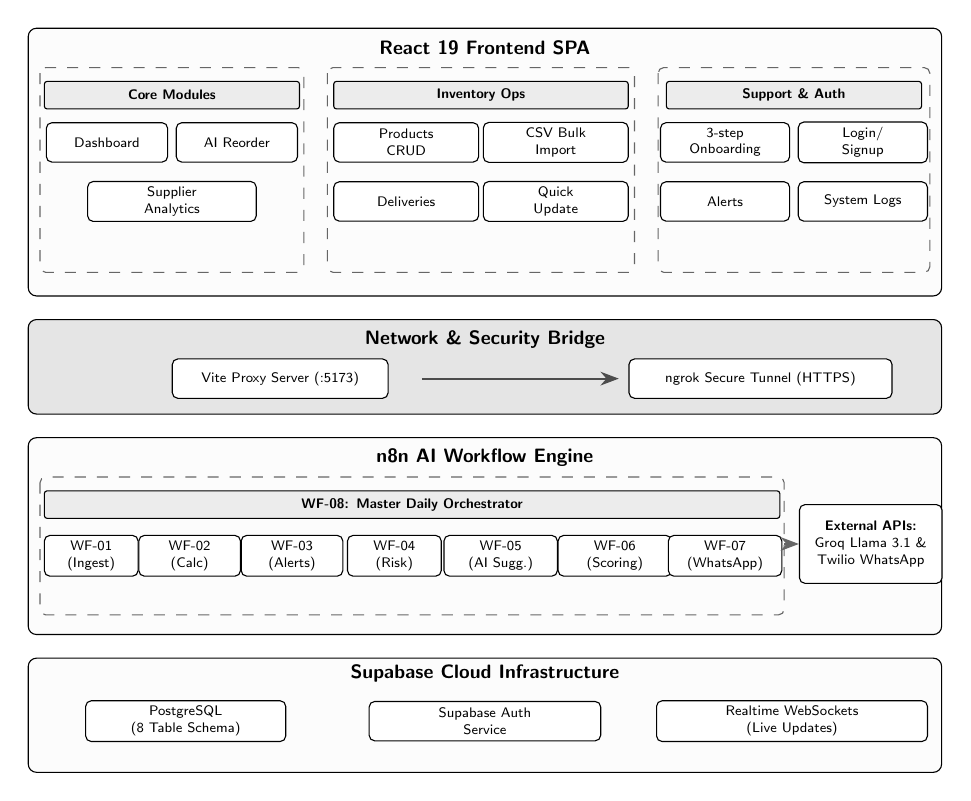
\begin{tikzpicture}[align=center,
  md/.style={rectangle, rounded corners=2pt, draw=black, fill=white,
    font=\sffamily\tiny, minimum height=0.5cm, text centered, inner sep=2pt},
  hd/.style={rectangle, rounded corners=1pt, draw=black, fill=gray!15, 
    font=\sffamily\tiny\bfseries, minimum height=0.35cm, text centered, inner sep=2pt},
]

% ====== LAYER 1: React 19 Frontend SPA ======
\draw[black, rounded corners=3pt, fill=gray!2] (0,0) rectangle (11.6,-3.4);
\node[font=\sffamily\scriptsize\bfseries] at (5.8,-0.25) {React 19 Frontend SPA};

% -- Core Modules --
\draw[black!60, rounded corners=2pt, dash pattern=on 4pt off 4pt] (0.15,-0.5) rectangle (3.5,-3.1);
\node[hd, text width=3.1cm] at (1.825,-0.85) {Core Modules};
\node[md, text width=1.4cm] at (1.0,-1.45) {Dashboard};
\node[md, text width=1.4cm] at (2.65,-1.45) {AI Reorder};
\node[md, text width=2.0cm] at (1.825,-2.2) {Supplier\\Analytics};

% -- Inventory Ops --
\draw[black!60, rounded corners=2pt, dash pattern=on 4pt off 4pt] (3.8,-0.5) rectangle (7.7,-3.1);
\node[hd, text width=3.6cm] at (5.75,-0.85) {Inventory Ops};
\node[md, text width=1.7cm] at (4.8,-1.45) {Products\\CRUD};
\node[md, text width=1.7cm] at (6.7,-1.45) {CSV Bulk\\Import};
\node[md, text width=1.7cm] at (4.8,-2.2) {Deliveries};
\node[md, text width=1.7cm] at (6.7,-2.2) {Quick\\Update};

% -- Support & Auth --
\draw[black!60, rounded corners=2pt, dash pattern=on 4pt off 4pt] (8.0,-0.5) rectangle (11.45,-3.1);
\node[hd, text width=3.1cm] at (9.725,-0.85) {Support \& Auth};
\node[md, text width=1.5cm] at (8.85,-1.45) {3-step\\Onboarding};
\node[md, text width=1.5cm] at (10.6,-1.45) {Login/\\Signup};
\node[md, text width=1.5cm] at (8.85,-2.2) {Alerts};
\node[md, text width=1.5cm] at (10.6,-2.2) {System Logs};

% ====== LAYER 2: Network & Security Bridge ======
\draw[black, rounded corners=3pt, fill=gray!20] (0,-3.7) rectangle (11.6,-4.9);
\node[font=\sffamily\scriptsize\bfseries] at (5.8,-3.95) {Network \& Security Bridge};
\node[md, text width=2.6cm] at (3.2,-4.45) {Vite Proxy Server (:5173)};
\draw[wf arrow] (5.0,-4.45) -- (7.5,-4.45);
\node[md, text width=3.2cm] at (9.3,-4.45) {ngrok Secure Tunnel (HTTPS)};

% ====== LAYER 3: n8n AI Workflow Engine ======
\draw[black, rounded corners=3pt, fill=gray!2] (0,-5.2) rectangle (11.6,-7.7);
\node[font=\sffamily\scriptsize\bfseries] at (5.8,-5.45) {n8n AI Workflow Engine};

% WF-08 Orchestrator sub-box
\draw[black!60, rounded corners=2pt, dash pattern=on 4pt off 4pt] (0.15,-5.7) rectangle (9.6,-7.45);
\node[hd, text width=9.2cm] at (4.875,-6.05) {WF-08: Master Daily Orchestrator};
\node[md, text width=1.05cm] at (0.8,-6.7) {WF-01\\(Ingest)};
\node[md, text width=1.15cm] at (2.05,-6.7) {WF-02\\(Calc)};
\node[md, text width=1.15cm] at (3.35,-6.7) {WF-03\\(Alerts)};
\node[md, text width=1.05cm] at (4.65,-6.7) {WF-04\\(Risk)};
\node[md, text width=1.3cm] at (6.0,-6.7) {WF-05\\(AI Sugg.)};
\node[md, text width=1.3cm] at (7.45,-6.7) {WF-06\\(Scoring)};
\node[md, text width=1.3cm] at (8.85,-6.7) {WF-07\\(WhatsApp)};

% External APIs box
\node[rectangle, draw=black, rounded corners=2pt, fill=white,
  font=\sffamily\tiny, text width=1.6cm, text centered, inner sep=3pt,
  minimum height=1.0cm] (api) at (10.7,-6.55)
  {\textbf{External APIs:}\\Groq Llama 3.1 \&\\Twilio WhatsApp};
\draw[wf arrow, black!60] (9.6,-6.55) -- (api.west);

% ====== LAYER 4: Supabase Cloud Infrastructure ======
\draw[black, rounded corners=3pt, fill=gray!2] (0,-8.0) rectangle (11.6,-9.45);
\node[font=\sffamily\scriptsize\bfseries] at (5.8,-8.2) {Supabase Cloud Infrastructure};
\node[md, text width=2.4cm] at (2.0,-8.8) {PostgreSQL\\(8 Table Schema)};
\node[md, text width=2.8cm] at (5.8,-8.8) {Supabase Auth\\Service};
\node[md, text width=3.3cm] at (9.7,-8.8) {Realtime WebSockets\\(Live Updates)};

\end{tikzpicture}%
}
\caption{StockSense AI System Architecture and Workflow Pipeline.}
\label{fig:workflow}
\end{figure}

\subsection{Mathematical Models}

The system implements several mathematical models for inventory analysis and supplier evaluation:

\textbf{Stockout Prediction Model (WF-02):}
The stockout date calculator computes the expected number of days until a product runs out of stock based on current inventory and sales velocity:

\begin{equation}
\label{eq:stockout_days}
d_{\text{stockout}} = \left\lfloor \frac{S_{\text{current}}}{V_{\text{daily}}} \right\rfloor
\end{equation}

\begin{equation}
\label{eq:stockout_date}
\text{date}_{\text{stockout}} = \text{date}_{\text{today}} + d_{\text{stockout}}
\end{equation}

where $S_{\text{current}}$ is the current stock level and $V_{\text{daily}}$ is the average daily sales velocity. If $V_{\text{daily}} = 0$, $d_{\text{stockout}}$ is set to 999 as a safe default. If $S_{\text{current}} = 0$, $d_{\text{stockout}} = 0$ indicating immediate stockout.

\textbf{Stock Risk Classification (WF-04):}
Products are classified into risk tiers based on $d_{\text{stockout}}$:

\begin{equation}
\label{eq:risk_classification}
\text{risk} =
\begin{cases}
\text{HIGH}    & \text{if } d_{\text{stockout}} \leq 3 \\
\text{MEDIUM}  & \text{if } 3 < d_{\text{stockout}} \leq 7 \\
\text{LOW}     & \text{if } d_{\text{stockout}} > 7 \\
\text{UNKNOWN} & \text{if no stockout data available}
\end{cases}
\end{equation}

\textbf{Supplier Scoring using Weighted Sum Model (WF-06):}
The supplier scoring system uses a multi-criteria Weighted Sum Model to compute a composite score for each supplier:

\begin{equation}
\label{eq:supplier_scoring}
C_s = (R \times 0.40 + P \times 0.35 + D \times 0.25) \times 100
\end{equation}

where $R$ is the reliability score (0--1 scale), $P$ is the price score (0--1 scale), and $D$ is the delivery speed score (min-max normalized: fastest supplier $= 1.0$, slowest $= 0.0$). Grade assignment follows: A if $C_s \geq 80$, B if $65 \leq C_s < 80$, C if $50 \leq C_s < 65$, D if $C_s < 50$.

\textbf{Inventory Health Score (Dashboard):}
The dashboard calculates an overall inventory health score:

\begin{equation}
\label{eq:health_score}
H = \min\!\left(100,\, \max\!\left(0,\, \left\lfloor \frac{\sum (n_i \cdot w_i)}{N} \right\rfloor\right)\right)
\end{equation}

where the numerator is $n_L \cdot 100 + n_M \cdot 70 + n_H \cdot 30 + n_O \cdot 5$, $n_L$, $n_M$, $n_H$, and $n_O$ are counts of LOW, MEDIUM, HIGH risk, and out-of-stock products respectively, and $N$ is the total number of products.

\section{Implementation}

\subsection{Tools and Technologies}
The technology choices were driven by two constraints: keep costs near zero and avoid anything that requires a dedicated backend developer. The frontend uses \textbf{React~19} with \textbf{Vite~8} for fast builds and \textbf{Tailwind CSS~v4} for styling. On the backend side, \textbf{Supabase} provides a managed PostgreSQL database with built-in auth and real-time WebSocket subscriptions---no separate server needed. All business logic lives inside \textbf{n8n}, a visual workflow engine that we self-host locally during development. For AI, the system calls the \textbf{Groq API} which hosts Llama~3.1~8B and returns inference results in under two seconds. \textbf{Twilio} handles the last mile: formatting a stock-alert message and delivering it over WhatsApp.

\subsection{Dataset}
We did not use a publicly available dataset. Instead, we synthesized a small catalog that mirrors a real kirana store: six fast-moving products (rice, atta, cooking oil, soap, biscuits, and dal) with realistic daily sales rates, reorder thresholds, and opening stock levels. Three supplier profiles were created with varying reliability and delivery-speed scores to exercise the WSM scoring logic. This controlled setup lets us test edge cases---for instance, what happens when a product has zero daily sales, or when stock is already at zero---without relying on noisy real-world data.

\subsection{Database Schema}

The Supabase PostgreSQL database contains eight tables as described in Table~\ref{tab:tables}.

\begin{table}[htbp]
\centering
\caption{Database Tables in StockSense AI}
\label{tab:tables}
\begin{tabular}{p{2.2cm}p{5.5cm}}
\toprule
\textbf{Table} & \textbf{Purpose} \\
\midrule
Store Profiles & Multi-tenancy-ready store configuration \\
Products & Inventory items with stock, pricing, risk \\
Suppliers & Vendor directory with scoring and grades \\
Stock Alerts & Low stock alerts (stock $\leq$ threshold) \\
Reorder Suggestions & AI-generated reorder recommendations \\
Stock Transactions & Audit log of all stock changes \\
Daily Snapshots & Historical daily health metrics \\
System Logs & Workflow execution logs \\
\bottomrule
\end{tabular}
\end{table}

All tables use UUID primary keys generated via \texttt{gen\_random\_uuid()}. The Products, Suppliers, Stock Alerts, and Reorder Suggestions tables include \texttt{store\_id} foreign keys for multi-tenancy-ready schema design. Indexes are created on frequently queried columns including \texttt{product\_id}, \texttt{risk\_level}, \texttt{alert\_status}, and \texttt{snapshot\_date}. Supabase Realtime subscriptions are enabled on Products, Stock Alerts, Reorder Suggestions, Daily Snapshots, and Suppliers tables for live frontend updates.

\subsection{Workflow Pipeline}

Eight n8n workflows implement the inventory intelligence pipeline.

\textbf{WF-01: Product and Sales Data Ingestion} exposes a POST webhook at \texttt{/product-sales-ingest} that receives product data from the frontend Add Product modal. The workflow validates and upserts products into the \textit{Products} table.

\begin{figure}[H]
\centering
\resizebox{\columnwidth}{!}{%
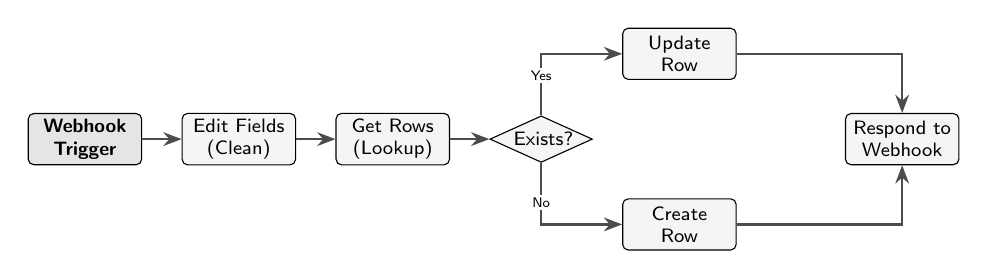
\begin{tikzpicture}[node distance=0.4cm and 0.5cm, align=center]
  \node (n1) [wf trigger] {Webhook\\Trigger};
  \node (n2) [wf node, right=of n1] {Edit Fields\\(Clean)};
  \node (n3) [wf node, right=of n2] {Get Rows\\(Lookup)};
  \node (n4) [wf decision, right=of n3] {Exists?};
  \node (n5a) [wf node, above right=0.6cm and 0.7cm of n4] {Update\\Row};
  \node (n5b) [wf node, below right=0.6cm and 0.7cm of n4] {Create\\Row};
  \node (n6) [wf node, right=3.2cm of n4] {Respond to\\Webhook};

  \draw [wf arrow] (n1) -- (n2);
  \draw [wf arrow] (n2) -- (n3);
  \draw [wf arrow] (n3) -- (n4);
  \draw [wf arrow] (n4) |- node[wf label, pos=0.25, above] {Yes} (n5a);
  \draw [wf arrow] (n4) |- node[wf label, pos=0.25, below] {No} (n5b);
  \draw [wf arrow] (n5a) -| (n6);
  \draw [wf arrow] (n5b) -| (n6);
\end{tikzpicture}}
\caption{WF-01: Data Ingestion Pipeline.}
\label{fig:wf01}
\end{figure}

\textbf{WF-02: Stockout Date Calculator} fetches all products, applies the stockout prediction formula from (\ref{eq:stockout_days}), and updates each product record with \texttt{days\_to\_stockout} and \texttt{estimated\_stockout\_date}.

\begin{figure}[H]
\centering
\resizebox{\columnwidth}{!}{%
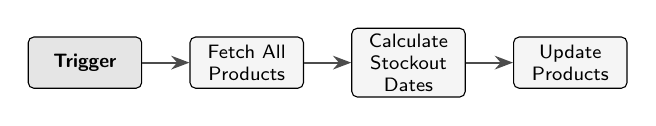
\begin{tikzpicture}[node distance=0.4cm and 0.6cm, align=center]
  \node (n1) [wf trigger] {Trigger};
  \node (n2) [wf node, right=of n1] {Fetch All\\Products};
  \node (n3) [wf node, right=of n2] {Calculate\\Stockout Dates};
  \node (n4) [wf node, right=of n3] {Update\\Products};

  \draw [wf arrow] (n1) -- (n2);
  \draw [wf arrow] (n2) -- (n3);
  \draw [wf arrow] (n3) -- (n4);
\end{tikzpicture}}
\caption{WF-02: Stockout Prediction Pipeline.}
\label{fig:wf02}
\end{figure}

\textbf{WF-03: Inventory Processing \& Stock Alerts} identifies products where \texttt{current\_stock} $\leq$ \texttt{reorder\_threshold}, clears existing alerts, and generates fresh \textit{Stock Alert} records.

\begin{figure}[H]
\centering
\resizebox{\columnwidth}{!}{%
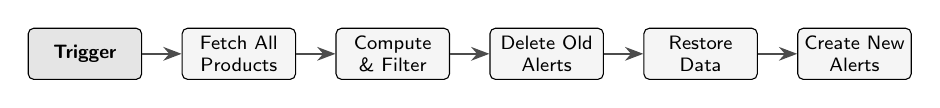
\begin{tikzpicture}[node distance=0.4cm and 0.5cm, align=center]
  \node (n1) [wf trigger] {Trigger};
  \node (n2) [wf node, right=of n1] {Fetch All\\Products};
  \node (n3) [wf node, right=of n2] {Compute\\\& Filter};
  \node (n4) [wf node, right=of n3] {Delete Old\\Alerts};
  \node (n5) [wf node, right=of n4] {Restore\\Data};
  \node (n6) [wf node, right=of n5] {Create New\\Alerts};

  \draw [wf arrow] (n1) -- (n2);
  \draw [wf arrow] (n2) -- (n3);
  \draw [wf arrow] (n3) -- (n4);
  \draw [wf arrow] (n4) -- (n5);
  \draw [wf arrow] (n5) -- (n6);
\end{tikzpicture}}
\caption{WF-03: Inventory Processing \& Alerts Pipeline.}
\label{fig:wf03}
\end{figure}

\textbf{WF-04: Stock Risk Classification} classifies all products into risk tiers using the formula in (\ref{eq:risk_classification}) based on \texttt{days\_to\_stockout} values from WF-02.

\begin{figure}[H]
\centering
\resizebox{\columnwidth}{!}{%
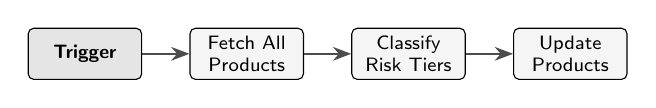
\begin{tikzpicture}[node distance=0.4cm and 0.6cm, align=center]
  \node (n1) [wf trigger] {Trigger};
  \node (n2) [wf node, right=of n1] {Fetch All\\Products};
  \node (n3) [wf node, right=of n2] {Classify\\Risk Tiers};
  \node (n4) [wf node, right=of n3] {Update\\Products};

  \draw [wf arrow] (n1) -- (n2);
  \draw [wf arrow] (n2) -- (n3);
  \draw [wf arrow] (n3) -- (n4);
\end{tikzpicture}}
\caption{WF-04: Risk Classification Pipeline.}
\label{fig:wf04}
\end{figure}

\textbf{WF-05: AI Reorder Intelligence} fetches at-risk products and all suppliers, then invokes Groq Llama 3.1 8B with a structured prompt to generate reorder recommendations. The LLM output is parsed and stored as \textit{Reorder Suggestions}.

\begin{figure}[H]
\centering
\resizebox{\columnwidth}{!}{%
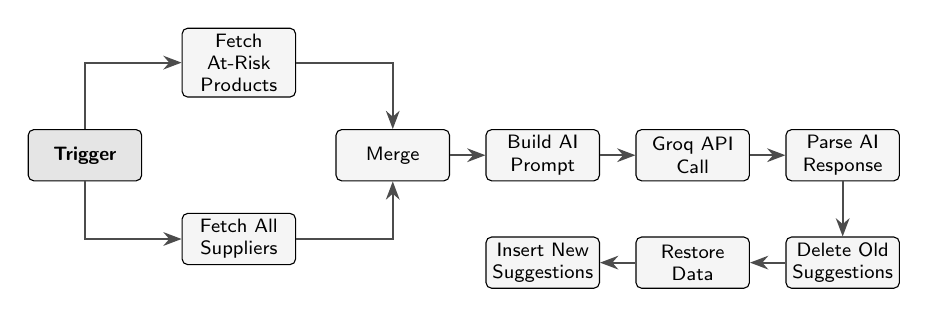
\begin{tikzpicture}[node distance=0.4cm and 0.45cm, align=center]
  % Row 1: Trigger -> parallel fetch -> merge -> prompt -> groq -> parse
  \node (n1) [wf trigger] {Trigger};
  \node (n2a) [wf node, above right=0.4cm and 0.5cm of n1] {Fetch At-Risk\\Products};
  \node (n2b) [wf node, below right=0.4cm and 0.5cm of n1] {Fetch All\\Suppliers};
  \node (n3) [wf node, below right=0.4cm and 0.5cm of n2a] {Merge};
  \node (n4) [wf node, right=of n3] {Build AI\\Prompt};
  \node (n5) [wf node, right=of n4] {Groq API\\Call};
  \node (n6) [wf node, right=of n5] {Parse AI\\Response};
  % Row 2: delete -> restore -> create
  \node (n7) [wf node, below=0.7cm of n6] {Delete Old\\Suggestions};
  \node (n8) [wf node, left=of n7] {Restore\\Data};
  \node (n9) [wf node, left=of n8] {Insert New\\Suggestions};

  \draw [wf arrow] (n1) |- (n2a);
  \draw [wf arrow] (n1) |- (n2b);
  \draw [wf arrow] (n2a) -| (n3);
  \draw [wf arrow] (n2b) -| (n3);
  \draw [wf arrow] (n3) -- (n4);
  \draw [wf arrow] (n4) -- (n5);
  \draw [wf arrow] (n5) -- (n6);
  \draw [wf arrow] (n6) -- (n7);
  \draw [wf arrow] (n7) -- (n8);
  \draw [wf arrow] (n8) -- (n9);
\end{tikzpicture}}
\caption{WF-05: AI Reorder Intelligence Pipeline.}
\label{fig:wf05}
\end{figure}

\textbf{WF-06: Supplier Scoring} evaluates all suppliers using the WSM formula from (\ref{eq:supplier_scoring}), computes composite scores, and assigns letter grades based on performance metrics.

\begin{figure}[H]
\centering
\resizebox{\columnwidth}{!}{%
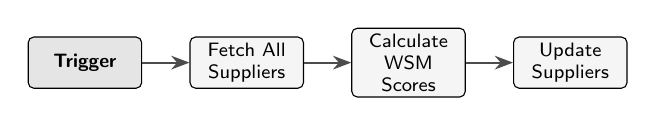
\begin{tikzpicture}[node distance=0.4cm and 0.6cm, align=center]
  \node (n1) [wf trigger] {Trigger};
  \node (n2) [wf node, right=of n1] {Fetch All\\Suppliers};
  \node (n3) [wf node, right=of n2] {Calculate\\WSM Scores};
  \node (n4) [wf node, right=of n3] {Update\\Suppliers};

  \draw [wf arrow] (n1) -- (n2);
  \draw [wf arrow] (n2) -- (n3);
  \draw [wf arrow] (n3) -- (n4);
\end{tikzpicture}}
\caption{WF-06: Supplier Scoring Pipeline.}
\label{fig:wf06}
\end{figure}

\textbf{WF-07: WhatsApp Alert Sender} queries active stock alerts, filters by 24-hour anti-spam cooldown, builds a formatted message, and delivers it via Twilio WhatsApp API.

\begin{figure}[H]
\centering
\resizebox{\columnwidth}{!}{%
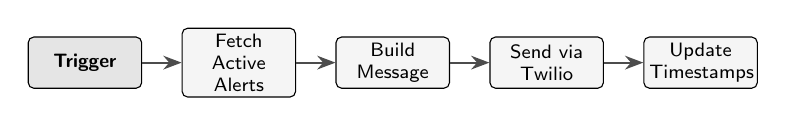
\begin{tikzpicture}[node distance=0.4cm and 0.5cm, align=center]
  \node (n1) [wf trigger] {Trigger};
  \node (n2) [wf node, right=of n1] {Fetch Active\\Alerts};
  \node (n3) [wf node, right=of n2] {Build\\Message};
  \node (n4) [wf node, right=of n3] {Send via\\Twilio};
  \node (n5) [wf node, right=of n4] {Update\\Timestamps};

  \draw [wf arrow] (n1) -- (n2);
  \draw [wf arrow] (n2) -- (n3);
  \draw [wf arrow] (n3) -- (n4);
  \draw [wf arrow] (n4) -- (n5);
\end{tikzpicture}}
\caption{WF-07: WhatsApp Alert Pipeline.}
\label{fig:wf07}
\end{figure}

\textbf{WF-08: Daily Orchestrator} is the master workflow executing at 8:00 AM IST. It simulates daily stock depletion, sequentially executes WF-02 through WF-07 as sub-workflows, computes and saves the daily health snapshot, and logs execution to \textit{System Logs}.

\begin{figure}[H]
\centering
\resizebox{\columnwidth}{!}{%
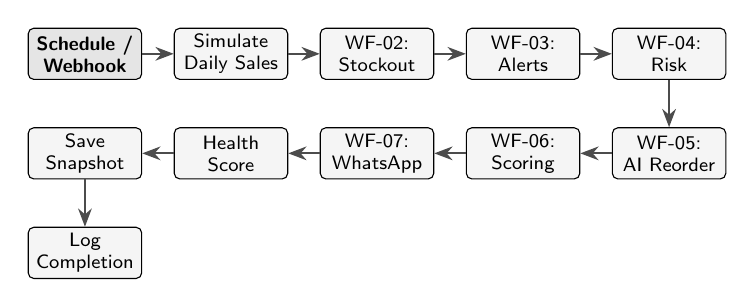
\begin{tikzpicture}[node distance=0.35cm and 0.4cm, align=center]
  % Row 1: Triggers -> Simulate -> WF-02 -> WF-03 -> WF-04
  \node (trig) [wf trigger] {Schedule /\\Webhook};
  \node (sim) [wf node, right=of trig] {Simulate\\Daily Sales};
  \node (w2) [wf node, right=of sim] {WF-02:\\Stockout};
  \node (w3) [wf node, right=of w2] {WF-03:\\Alerts};
  \node (w4) [wf node, right=of w3] {WF-04:\\Risk};
  % Row 2: WF-05 -> WF-06 -> WF-07 -> Snapshot -> Log
  \node (w5) [wf node, below=0.6cm of w4] {WF-05:\\AI Reorder};
  \node (w6) [wf node, left=of w5] {WF-06:\\Scoring};
  \node (w7) [wf node, left=of w6] {WF-07:\\WhatsApp};
  \node (score) [wf node, left=of w7] {Health\\Score};
  \node (snap) [wf node, left=of score] {Save\\Snapshot};
  % Row 3
  \node (log) [wf node, below=0.6cm of snap] {Log\\Completion};

  \draw [wf arrow] (trig) -- (sim);
  \draw [wf arrow] (sim) -- (w2);
  \draw [wf arrow] (w2) -- (w3);
  \draw [wf arrow] (w3) -- (w4);
  \draw [wf arrow] (w4) -- (w5);
  \draw [wf arrow] (w5) -- (w6);
  \draw [wf arrow] (w6) -- (w7);
  \draw [wf arrow] (w7) -- (score);
  \draw [wf arrow] (score) -- (snap);
  \draw [wf arrow] (snap) -- (log);
\end{tikzpicture}}
\caption{WF-08: Master Daily Orchestrator Pipeline.}
\label{fig:wf08}
\end{figure}

\newpage
\subsection{LLM Prompt Engineering}

WF-05 constructs a structured prompt submitted to the 
Groq Llama~3.1~8B inference endpoint. The prompt 
follows a zero-shot instruction format comprising three 
components: (1)~a role definition establishing the 
model as an inventory manager for an Indian kirana store; 
(2)~structured context blocks listing at-risk products 
with fields \texttt{product\_id}, \texttt{category}, 
\texttt{current\_stock}, \texttt{avg\_daily\_sales}, 
\texttt{days\_to\_stockout}, and \texttt{risk\_level}; 
and (3)~available supplier profiles with 
\texttt{supplier\_id}, \texttt{supplier\_grade}, 
\texttt{delivery\_time\_days}, and 
\texttt{supplies\_categories}.

The model is instructed to return a JSON array only, 
with no markdown fencing or natural language preamble. 
Each element contains \texttt{product\_id}, 
\texttt{supplier\_id}, \texttt{suggested\_quantity} 
(computed as $30 \times v$ where $v$ is average daily 
sales), and a \texttt{reason} field providing a 
single-sentence justification. Category matching between 
products and supplier inventories is enforced as 
case-insensitive. A rule-based fallback activates 
if the API response cannot be parsed as valid JSON, 
ensuring the system remains operational during 
inference failures.

\subsection{Frontend Application}

The React 19 frontend provides 12 routes as described in Table~\ref{tab:routes}.

\begin{table}[htbp]
\centering
\caption{Frontend Routes and Functions}
\label{tab:routes}
\begin{tabular}{p{2.2cm}p{5.5cm}}
\toprule
\textbf{Route} & \textbf{Function} \\
\midrule
/ & Landing page \\
/login, /signup & Supabase Auth entry points \\
/reset-password & Password reset flow \\
/onboarding & 3-step store setup wizard \\
/dashboard & Health score, KPIs, critical products, trend chart \\
/products & Product CRUD with CSV bulk import \\
/quick-update & Batch stock adjustments \\
/alerts & Stock alert feed with dismiss \\
/reorder & AI reorder suggestions with approve/dismiss \\
/suppliers & Supplier table with grade badges \\
/logs & System log viewer \\
/settings & Store profile and workflow triggers \\
\bottomrule
\end{tabular}
\end{table}

The Dashboard implements a real-time pipeline overlay: when the user triggers WF-08, an animated modal cycles through realistic step messages while a Supabase Realtime subscription on System Logs listens for the pipeline completion insert. The moment n8n finishes, the overlay closes and the dashboard refreshes automatically without polling.

\section{Results and Performance}


The system was tested end-to-end with six products and three suppliers. Table~\ref{tab:perf} lists the key numbers.

\begin{table}[htbp]
\centering
\caption{System Performance Metrics}
\label{tab:perf}
\begin{tabular}{lc}
\toprule
\textbf{Metric} & \textbf{Value} \\
\midrule
Number of Workflows & 8 \\
Number of Database Tables & 8 \\
Number of Frontend Routes & 12 \\
Pipeline Execution Time & $\sim$13 seconds \\
WhatsApp Message Delivery & $<$5 seconds \\
Infrastructure Cost & Rs.\ 0 (prototype); $<$Rs.\ 500/mo (production) \\
\bottomrule
\end{tabular}
\end{table}

Table IV puts StockSense side by side with three apps that Indian retailers commonly use today. The main takeaway is that none of the alternatives offer AI-based reorder logic or automated WhatsApp alerts at a comparable price point.

\begin{table}[htbp]
\centering
\caption{Comparison with Existing Inventory Solutions}
\label{tab:comparison}
\renewcommand{\arraystretch}{1.4}
\begin{tabularx}{\columnwidth}{lXXXX}
\toprule
\textbf{Feature} & \textbf{StockSense AI} & \textbf{Vyapar} & \textbf{Zoho Inventory} & \textbf{Khatabook} \\
\midrule
AI Reorder Suggestions & Yes & No & Limited & No \\
Stockout Prediction & Automated & Manual & Basic & No \\
Supplier Scoring & WSM-based & No & Basic & No \\
WhatsApp Alerts & Automated & No & No & No \\
Monthly Cost & Rs. 0--500 & Rs. 0--599 & Rs. 4,000+ & Rs. 0 \\
Setup Complexity & Low & Medium & High & Low \\
Prediction Method & Rule-based & No & Basic & No \\
Real-time Dashboard & Yes & Limited & Yes & No \\
\bottomrule
\end{tabularx}
\end{table}

\subsection*{Health Score Validation}
To make sure the health-score formula from~(5) behaves sensibly, we ran it against four inventory states that a kirana store might realistically encounter. Table~V shows the results.

\begin{table}[htbp]
\centering
\caption{Health Score Across Inventory States}
\label{tab:healthscores}
\renewcommand{\arraystretch}{1.4}
\begin{tabular}{lcccccc}
\toprule
\textbf{Scenario} & $n_L$ & $n_M$ & $n_H$ & $n_O$ & $N$ & $H$ \\
\midrule
All well-stocked   & 6 & 0 & 0 & 0 & 6 & 100 \\
Demo state         & 1 & 2 & 3 & 0 & 6 & 55  \\
Partial stockout   & 0 & 1 & 2 & 3 & 6 & 18  \\
Complete stockout  & 0 & 0 & 0 & 6 & 6 & 5   \\
\bottomrule
\end{tabular}
\end{table}

The numbers make intuitive sense. A store with everything in stock gets a perfect 100; the demo dataset (three high-risk items) lands at 55; and a store where three products are completely out scores just 18, which would trigger an urgent alert. We deliberately set the floor at 5 instead of 0 so that the dashboard gauge never shows a completely empty reading, which could confuse the user into thinking the system is broken.

On the cost side, the prototype runs entirely on free tiers: Supabase gives 500~MB of PostgreSQL storage, Groq offers rate-limited LLM inference at no charge, and n8n runs on the developer's laptop. Twilio WhatsApp works in sandbox mode during testing. Moving to production would require hosting n8n on a cloud platform like Railway or Render (roughly Rs.~300--500 per month) and paying Twilio's per-message fees. Even so, the total monthly bill for one store stays well below Rs.~500, which is an order of magnitude cheaper than Zoho Inventory.

The daily pipeline ran without errors across multiple test cycles. Each morning at 8:00~AM, n8n's cron trigger kicks off the master workflow, and all eight sub-pipelines execute in sequence. The only caveat is that this schedule only works while the n8n instance is actually running and reachable.

WhatsApp turned out to be the right delivery channel. Indian shopkeepers check WhatsApp far more often than email, and the built-in 24-hour cooldown we added prevents the same alert from being sent repeatedly. During testing, messages arrived consistently within five seconds of the pipeline finishing.

The health score proved useful as a single-glance metric. Rather than scanning a table of six products, the owner sees one number on the dashboard and immediately knows whether to worry.

The AI reorder suggestions were the most interesting part to evaluate. Groq Llama~3.1~8B takes the product list, the supplier profiles, and the risk levels, and returns a JSON array with quantity suggestions and a one-line justification for each. The reasoning is not always perfect---occasionally the model suggests ordering from a supplier who does not carry that category---but the rule-based fallback catches these cases and defaults to a $30 \times v$ formula.

\section{Conclusion}

StockSense AI set out to answer a simple question: can a small Indian shopkeeper get useful inventory intelligence without paying enterprise prices? Based on our prototype, the answer is a cautious yes. The system automates the entire loop---from tracking stock levels to sending a WhatsApp message that says ``order 30 packets of Aashirvaad Atta from Supplier~A''---and it does so for under Rs.~500 a month in production.

That said, several limitations remain. The stockout prediction is rule-based, not learned from data, so it cannot account for demand surges during festivals. The LLM occasionally produces malformed output, which the fallback catches but does not improve upon. And the 8:00~AM schedule only works if the n8n instance is online, which requires cloud hosting that a non-technical owner cannot manage alone.

\section{Future Scope}

\label{sec:future}

The current version is a working baseline. Below are the extensions we consider most impactful.

\textbf{Barcode Scanning:} Right now, products are added by typing in details manually. Hooking into the phone camera for barcode or QR lookups would cut onboarding time significantly. The existing \texttt{product\_id} field already accepts barcode strings, so no schema change is needed.

\textbf{Voice Input in Regional Languages:} Many kirana owners are more comfortable speaking than typing. A voice interface accepting Telugu, Hindi, or Marathi commands like ``5 packet Aashirvaad Atta aaya'' would make stock updates much faster. The Web Speech API is browser-native and would not add infrastructure cost.

\textbf{Two-way WhatsApp:} Currently, WhatsApp is one-directional---the system sends alerts, but the owner cannot reply to approve a reorder. Wiring up a Twilio inbound webhook would let owners respond with ``yes'' or ``no'' directly from the chat, removing the need to open the dashboard.

\textbf{Seasonal Adjustments:} The Products table already has \texttt{is\_seasonal} and \texttt{peak\_season\_months} columns that are not yet active. Turning them on would let the system multiply \texttt{avg\_daily\_sales} by a seasonal factor before Diwali or Holi, improving stockout predictions during peak demand.

\textbf{Multi-store Support:} The schema includes a \texttt{store\_id} foreign key in every table, so the database is already multi-tenancy-ready. Adding Supabase Row Level Security policies scoped to \texttt{store\_id} would let multiple stores share one deployment without seeing each other's data.

\textbf{Purchase Orders:} Once a reorder suggestion is approved, the next logical step is generating a formal purchase order with a UPI payment link. This would close the procurement loop entirely within the app.

\begin{thebibliography}{10}

\bibitem{inventory2024}
J. Wang, P. Li, L. Luo and H . Sun, ``Design and Development of Intelligent Inventory System for Small and Micro Enterprise Warehousing,'' \emph{IEEE Conf. on Computer, Big Data and AI}, 2024. [Online]. Available: \url{https://ieeexplore.ieee.org/document/10550978/}

\bibitem{forecasting2023}
N. Kheawpeam and S. Sinthupinyo, ``Demand Forecasting Using Machine Learning to Manage Product Inventory for Multi-channel Retailing Store,'' \emph{IEEE Int. Conf. on Omni-layer Intelligent Systems}, 2023. [Online]. Available: \url{https://ieeexplore.ieee.org/document/10189241/}

\bibitem{retail2024}
Jaymin V. Soni and Chetansinh Vaghela, ``Retail Demand Forecasting in Inventory with External Influences: A Comparative Study of Machine Learning Models,'' \emph{IEEE Trans. on Retail Tech.}, 2024. [Online]. Available: \url{https://ieeexplore.ieee.org/document/11232957/}

\bibitem{llm2024}
Mohammad Al Khaldy and Youcef Gheraibia, ``Evaluation and Mitigation of the Limitations of Large Language Models in Business Decision-Making,'' \emph{IEEE Access}, 2024. [Online]. Available: \url{https://ieeexplore.ieee.org/document/11013278/}

\bibitem{cognitive2025}
Natalie Friedman, Marcus Krug. and S. Joy Mountford, ``Mediating Cognitive Biases in Business Decisions Using LLMs,'' \emph{IEEE Trans. on AI}, 2025. [Online]. Available: \url{https://ieeexplore.ieee.org/document/11050471/}

\bibitem{workflow2025}
Ahmed Raza Amir and Syed Muhammad Atif, ``Evaluating Workflow Automation Efficiency Using n8n: A Small-Scale Business Case Study,'' \emph{arXiv preprint arXiv:2602.01311}, Feb. 2025. [Online]. Available: \url{https://arxiv.org/abs/2602.01311}

\bibitem{msme2019}
Dinesh Shenoy and Hoshiar Mal, ``A Multi-item Inventory Model for Small Business---A Perspective from India,'' \emph{Int. J. of Inventory Research}, vol.~5, no.~3, pp.~188--209, 2019. [Online]. Available: \url{https://www.inderscienceonline.com/doi/abs/10.1504/IJIR.2019.098856}

\bibitem{iot2024}
Geetha Manoharan, Vipin Kumar, A Karthik, V Asha, Chinnem Rama Mohan, and Ginni Nijhawan, ``IoT-Based Smart Inventory Management System Using Machine Learning Techniques,'' \emph{IEEE Internet of Things Journal}, 2024. [Online]. Available: \url{https://ieeexplore.ieee.org/document/10601903/}

\bibitem{smartretail2024}
K. Poongothai, Devika. G, Sweety Brisila. D, and Yogesh. S, ``Smart Retail Using Machine Learning for Demand Forecasting and Inventory Optimization,'' \emph{IEEE Trans. on Smart Business}, 2024. [Online]. Available: \url{https://ieeexplore.ieee.org/document/10910874/}

\bibitem{n8n2025}
Padmanabhan Venkiteela, ``n8n: An Open-Source Workflow Automation Platform for Enterprise Integration and AI-Driven Orchestration,'' \emph{Int. J. of Computer Applications}, vol.~187, no.~63, Dec.~2025. [Online]. Available: \url{https://www.ijcaonline.org/archives/volume187/number63/}

\end{thebibliography}

\end{document}